\documentclass[11pt]{ctexart}

\usepackage[margin=2cm,a4paper]{geometry}
\setmainfont{Caladea}
%% 也可以选用其它字库:
% \setCJKmainfont[%
%   ItalicFont=AR PL KaitiM GB,
%   BoldFont=Noto Sans CJK SC,
% ]{Noto Serif CJK SC}
% \setCJKsansfont{Noto Sans CJK SC}
% \renewcommand{\kaishu}{\CJKfontspec{AR PL KaitiM GB}}

\usepackage{minted}
\usepackage[breaklinks]{hyperref}

% Picture
% 导言区的此三行无变化
\usepackage{graphicx}
\usepackage{float} 
\usepackage{subfigure}
% 以下是新增的自定义格式更改
\usepackage[]{caption2} %新增调用的宏包
\renewcommand{\figurename}{Fig.} %重定义编号前缀词
\renewcommand{\captionlabeldelim}{.~} %重定义分隔符
 %\roman 是罗马数字编号,\alph是默认的字母编号,\arabic是阿拉伯数字编号,可按需替换下一行的相应位置
\renewcommand{\thesubfigure}{(\roman{subfigure})}%此外,还可设置图编号显示格式,加括号或者不加括号
\makeatletter \renewcommand{\@thesubfigure}{\thesubfigure \space}%子图编号与名称的间隔设置
\renewcommand{\p@subfigure}{} \makeatother

% Math
\usepackage {mathtools}

% Code
\usepackage{listings}
\usepackage{xcolor}
\lstset{
    % backgroundcolor=\color{red!50!green!50!blue!50},
    % 程式碼塊背景色為淺灰色
    rulesepcolor= \color{gray}, % 程式碼塊邊框顏色
    breaklines=true,  % 程式碼過長則換行
    numbers=left, % 行號在左側顯示
    numberstyle= \small,% 行號字型
    % eywordstyle= \color{red,% 關鍵字顏色
    commentstyle=\color{gray}, % 註釋顏色
    frame=shadowbox % 用方框框住程式碼塊
    }


\title{報告模板}
\author{干皓丞}

\begin{document}
\maketitle

程式碼
	\begin{lstlisting}[language={java}]
// Java code
public class Main{
	public static void main(String[]args){
		System.out.println("hello,world");
	}
}
	\end{lstlisting}


Overleaf 伺服器上安装的字体都是开源授权的,因此很多C\TeX{}模板设定的默认字体都不能使用(都是微软视窗或Adobe字体)。导致有些朋友上载了自己的C\TeX{}文件却不能编译,抓狂不已。

其实最重要的是,不要用 \verb|fontset=windows|!伺服器上没有 Windows 字体,真的有需要的话,请自行上传 .ttf 文件。

其实无需再加任何 \verb|fontset| 选项,系统会在 XeLaTeX 或 LuaLaTeX 下自动调用 Fandol,编译、显示都没有问题。调用效果如下:

\begin{itemize}
\item 一般字体(\verb|\rmfamily|)为〖宋体〗。
\item 需要强调时,Fandol \verb|\textbf| 用的是〖\textbf{加黑宋体}〗。
\item \verb|\sffamily| 用的是 〖\textsf{黑体}〗。
\item 中文字体是没有斜体的,因此 \verb|\emph|和 \verb|\textit| 都是〖\textit{楷体}〗。

\item 单距字体(\verb|\ttfamily|)很多人爱用\texttt{〖仿宋〗}。

\end{itemize}


想调用其它字库的话,伺服器上现有的中文字库可参考这个列表:\url{https://www.overleaf.com/help/193#!CJK}。

也可以自行上载 TTF/OTF 档案,直接用档案名来,如:\mintinline{LaTeX}{\setmainfont{shuti.otf}}。目前伺服器上没有幼圆、隶书字库可供C\TeX{}直接使用,抱歉了。


繁体的话,先用\verb|nofonts|参数,再用\verb|fontspec|方法来配置字库。可以考虑 cwTeXKai, cwTeXMing, cwTeXHeiBold, cwTeXYen, Noto Serif CJK TC, Noto Sans CJK TC。比如:

\begin{minted}{LaTeX}
\documentclass[nofonts]{ctexart}
\setCJKmainfont[
  BoldFont={cwTeXHeiBold},
  ItalicFont={cwTeXKai}]
{cwTeXMing}
\setCJKsansfont{cwTeXHei}
\setCJKmonofont{cwTeXYen}
\end{minted}

\begin{figure}[H]
\centering 
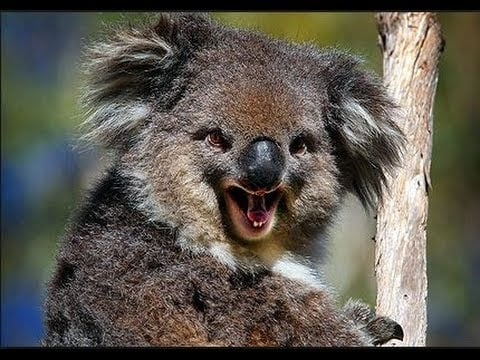
\includegraphics[width=0.7\textwidth]{test.jpg} 
\caption{Figure 2}
\label{Report.2}
\end{figure}

% 注意:此段中在引用中增加了主图编号的引用
Figure \ref{Fig.main} has two sub-figures, fig. \ref{Fig.main}\ref{Fig.sub.1} is the travel demand of driving auto, and fig. \ref{Fig.main}\ref{Fig.sub.2} is the travel demand of park-and-ride.
%以下code与上一小结的无变化
\begin{figure}[H]
\centering  %图片全局居中
\subfigure[name1]{
\label{Fig.sub.1}
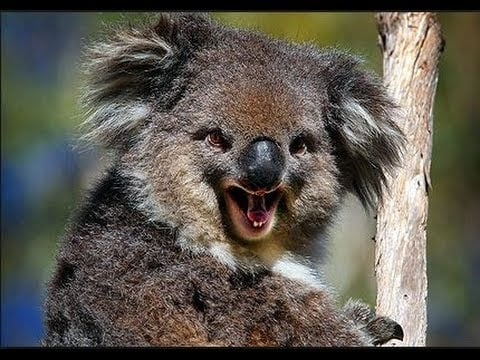
\includegraphics[width=0.45\textwidth]{test.jpg}}
\subfigure[name2]{
\label{Fig.sub.2}
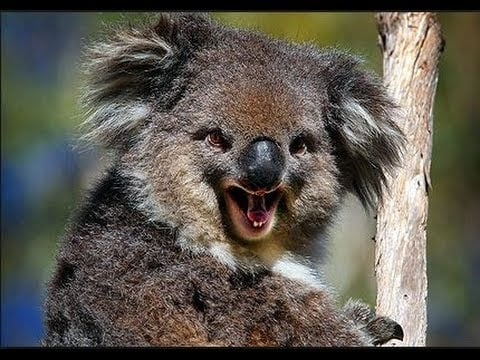
\includegraphics[width=0.45\textwidth]{test.jpg}}
\caption{Main name}
\label{Fig.main}
\end{figure}

$$\sum_{i=1}^n a_i=0$$
$$\sin{\alpha}\pm\sin{\beta}=2\sin{\frac{1}{2}\left(\alpha\pm\beta\right)}\cos{\frac{1}{2}\left(\alpha\mp\beta\right)}$$

\end{document}